\documentclass[11pt]{article}
\usepackage[margin=1in]{geometry}
\usepackage{amsmath,amssymb}
\usepackage{booktabs}
\usepackage{siunitx}
\usepackage{hyperref}
\usepackage{graphicx}
\usepackage{epstopdf}
\usepackage{caption}
\usepackage{xcolor}

\sisetup{
  separate-uncertainty = true,
  per-mode = symbol,
}

\title{W8: Hybrid FELsim/RF-Track Stage~11 Optimisation}
\author{Eremey Valetov}
\date{24 February 2026}

\begin{document}
\maketitle

\section{Objective}

Optimise Stage~11 of the UH MkV FEL beamline using RF-Track particle tracking
instead of FELsim's linear transfer matrices.  The goal is twofold: (a)~validate
the transfer matrix model against full nonlinear particle tracking, and
(b)~determine whether RF-Track can achieve a better undulator Twiss match by
capturing effects absent from the linear model (space charge, higher-order optics,
realistic dipole transport).

This study complements the COSY cross-validation (W4), which compared
gradient-based and gradient-free \emph{matrix} optimisers.  Here we compare
a \emph{matrix} optimiser (FELsim) against a \emph{particle tracking} optimiser
(RF-Track) on the same problem.


\section{Method}

\subsection{Hybrid Approach}

Stages~1--10 are fast, local matches (1--4 variables each, small beamline
segments) where linear transfer matrices are adequate.  Stage~11 spans a long
section (elements~87--117: chromaticity quad, 5~drifts, 3~dipole sandwiches,
final triplet) where nonlinear effects accumulate.  The hybrid approach runs
FELsim for Stages~1--10 and RF-Track for Stage~11:

\begin{enumerate}
  \item Run the full 11-stage FELsim optimisation (NM, 5 restarts for Stage~11).
  \item Extract all 23 quad currents from the FELsim result.
  \item Build the RF-Track lattice with those currents.
  \item Re-optimise Stage~11 variables (quads 87, 93, 95, 97) using
    Nelder-Mead with the RF-Track objective function.
\end{enumerate}

\subsection{RF-Track Objective Function}

Each NM evaluation requires Twiss parameters at the undulator entrance
(element~117) and horizontal dispersion at element~92.  Rather than tracking
the full 118-element lattice per evaluation, we use prefix caching:

\begin{itemize}
  \item \textbf{Prefix (once):} Track 500 particles from element~0 through
    element~87 (all elements upstream of Stage~11).  This takes
    $\approx$\SI{0.2}{s} and is performed once before the optimisation loop.
  \item \textbf{Suffix (per eval):} From the cached prefix state, track two
    sub-lattices: elements~87--93 (for dispersion at element~92) and
    elements~87--118 (for final Twiss).  Each suffix tracking takes
    $\approx$\SI{0.1}{s}.
\end{itemize}

The MSE is the same 5-term formula used by FELsim:
\begin{equation}
  \text{MSE} = \frac{1}{5}\Bigl[
    \tfrac{1}{2}\,\eta_x(92)^2
    + (\alpha_x - 0.470)^2
    + \alpha_y^2
    + (\beta_x - 1.400)^2
    + (\beta_y - 0.242)^2
  \Bigr],
\end{equation}
where Twiss parameters and dispersion are computed from the tracked particle
distribution using statistical moments.

\subsection{Multi-Start Configuration}

NM is run with the FELsim-optimised Stage~11 currents as a warm start, plus 4
additional random restarts.  Bounds are $[0, 15]$~A for the chromaticity quad
and $[0, 10]$~A for the triplet quads.  Beam: $E = \SI{40}{MeV}$,
$\sigma_E = 0.5\%$, $\varepsilon_n = 8\;\pi\cdot\text{mm}\cdot\text{mrad}$,
500~particles, seed = 42.


\section{Adapter Fixes}

Two issues in the RF-Track adapter were identified and resolved during
element-by-element comparison with FELsim.

\subsection{DIPOLE\_WEDGE as Zero-Length Drift}

FELsim models dipole wedges (\texttt{DIPOLE\_WEDGE}) as thin-lens edge kicks:
the transfer matrix is identity in $x$ with a small $y$-kick from the
fringe field integral.  The RF-Track adapter was converting these to
\texttt{Drift(length)} with the physical wedge length ($\approx$\SI{10}{mm}),
adding spurious position propagation ($x \mathrel{+}= L\,x'$) at every
dipole edge.

Fix: \texttt{DIPOLE\_WEDGE} $\to$ \texttt{Drift(0)}.  After this change,
element-by-element comparison with FELsim agrees to 4+ decimal places through
drifts and quadrupoles.  Residual differences at dipoles are expected (RF-Track
uses a sector bend model; FELsim uses a matrix model with a triangle-rule
fringe correction).

\subsection{Quadrupole \texttt{set\_strength()} Verification}

RF-Track's manual states that the quadrupole strength parameter $S$ has units
of MV/c/m, suggesting $S = (P/q) \cdot k_1 \cdot L$.  A single-quad
benchmark showed that \texttt{set\_strength(k1 * L)} reproduces FELsim's
transfer matrix exactly, while \texttt{set\_K1(Pc, k1)} or
\texttt{set\_gradient(G)} produce excessively strong focusing that loses all
particles.  The internal tracking evidently uses $S/L$ as the effective $k_1$,
\emph{not} $S/(P_Q \cdot L)$.  The original adapter code was confirmed correct.


\section{Results}

Three configurations are compared at $\varepsilon_n = 8$:
\begin{description}
  \item[FELsim] Full 11-stage NM optimisation using transfer matrices.
  \item[RFT-val] RF-Track lattice evaluated with FELsim-optimised currents
    (no re-optimisation --- measures how well FELsim currents transfer to
    a particle tracking code).
  \item[RFT-opt] RF-Track Stage~11 NM optimisation (hybrid approach).
\end{description}

\begin{table}[ht]
\centering
\caption{Twiss comparison at $\varepsilon_n = 8$.  Targets:
  $\beta_x = \SI{1.400}{m}$, $\beta_y = \SI{0.242}{m}$,
  $\alpha_x = 0.470$, $\alpha_y = 0$.}
\label{tab:twiss}
\begin{tabular}{@{} l S[scientific-notation=true] S S S S S @{}}
\toprule
{Method} & {MSE} & {$\alpha_x$} & {$\alpha_y$} & {$\beta_x$ (m)} & {$\beta_y$ (m)}
  & {$\eta_x$(92) (m)} \\
\midrule
FELsim  & 8.08e-04 &   0.471 & -0.005 &  1.399 & 0.304 & 0.015 \\
RFT-val & 2.55e+03 & -74.009 & -3.029 & 86.278 & 0.987 & 0.007 \\
RFT-opt & 6.43e-06 &   0.469 &  0.000 &  1.401 & 0.246 & 0.005 \\
\bottomrule
\end{tabular}
\end{table}

\begin{table}[ht]
\centering
\caption{Stage~11 quad currents and performance.  FELsim and RFT-val share
  the same currents; RFT-opt finds a qualitatively different solution.}
\label{tab:currents}
\begin{tabular}{@{} l SSSS SS @{}}
\toprule
{Method} & {$I_{87}$ (A)} & {$I_{93}$ (A)} & {$I_{95}$ (A)} & {$I_{97}$ (A)}
  & {nfev} & {Time (s)} \\
\midrule
FELsim  & 1.60 & 1.43 & 2.89 & 1.92 & 371 & 82.4 \\
RFT-val & 1.60 & 1.43 & 2.89 & 1.92 &   0 &  0.9 \\
RFT-opt & 2.05 & 1.41 & 0.72 & 0.11 & 656 & 80.3 \\
\bottomrule
\end{tabular}
\end{table}

\begin{figure}[ht]
\centering

\includegraphics[width=0.85\textwidth]{results/rftrack_opt/mse_comparison.pdf}
\caption{MSE comparison (log scale).  RFT-opt achieves $125\times$ lower MSE
  than FELsim.  RFT-val (FELsim currents in RF-Track) produces wildly
  incorrect optics.}
\label{fig:mse}
\end{figure}

\begin{figure}[ht]
\centering
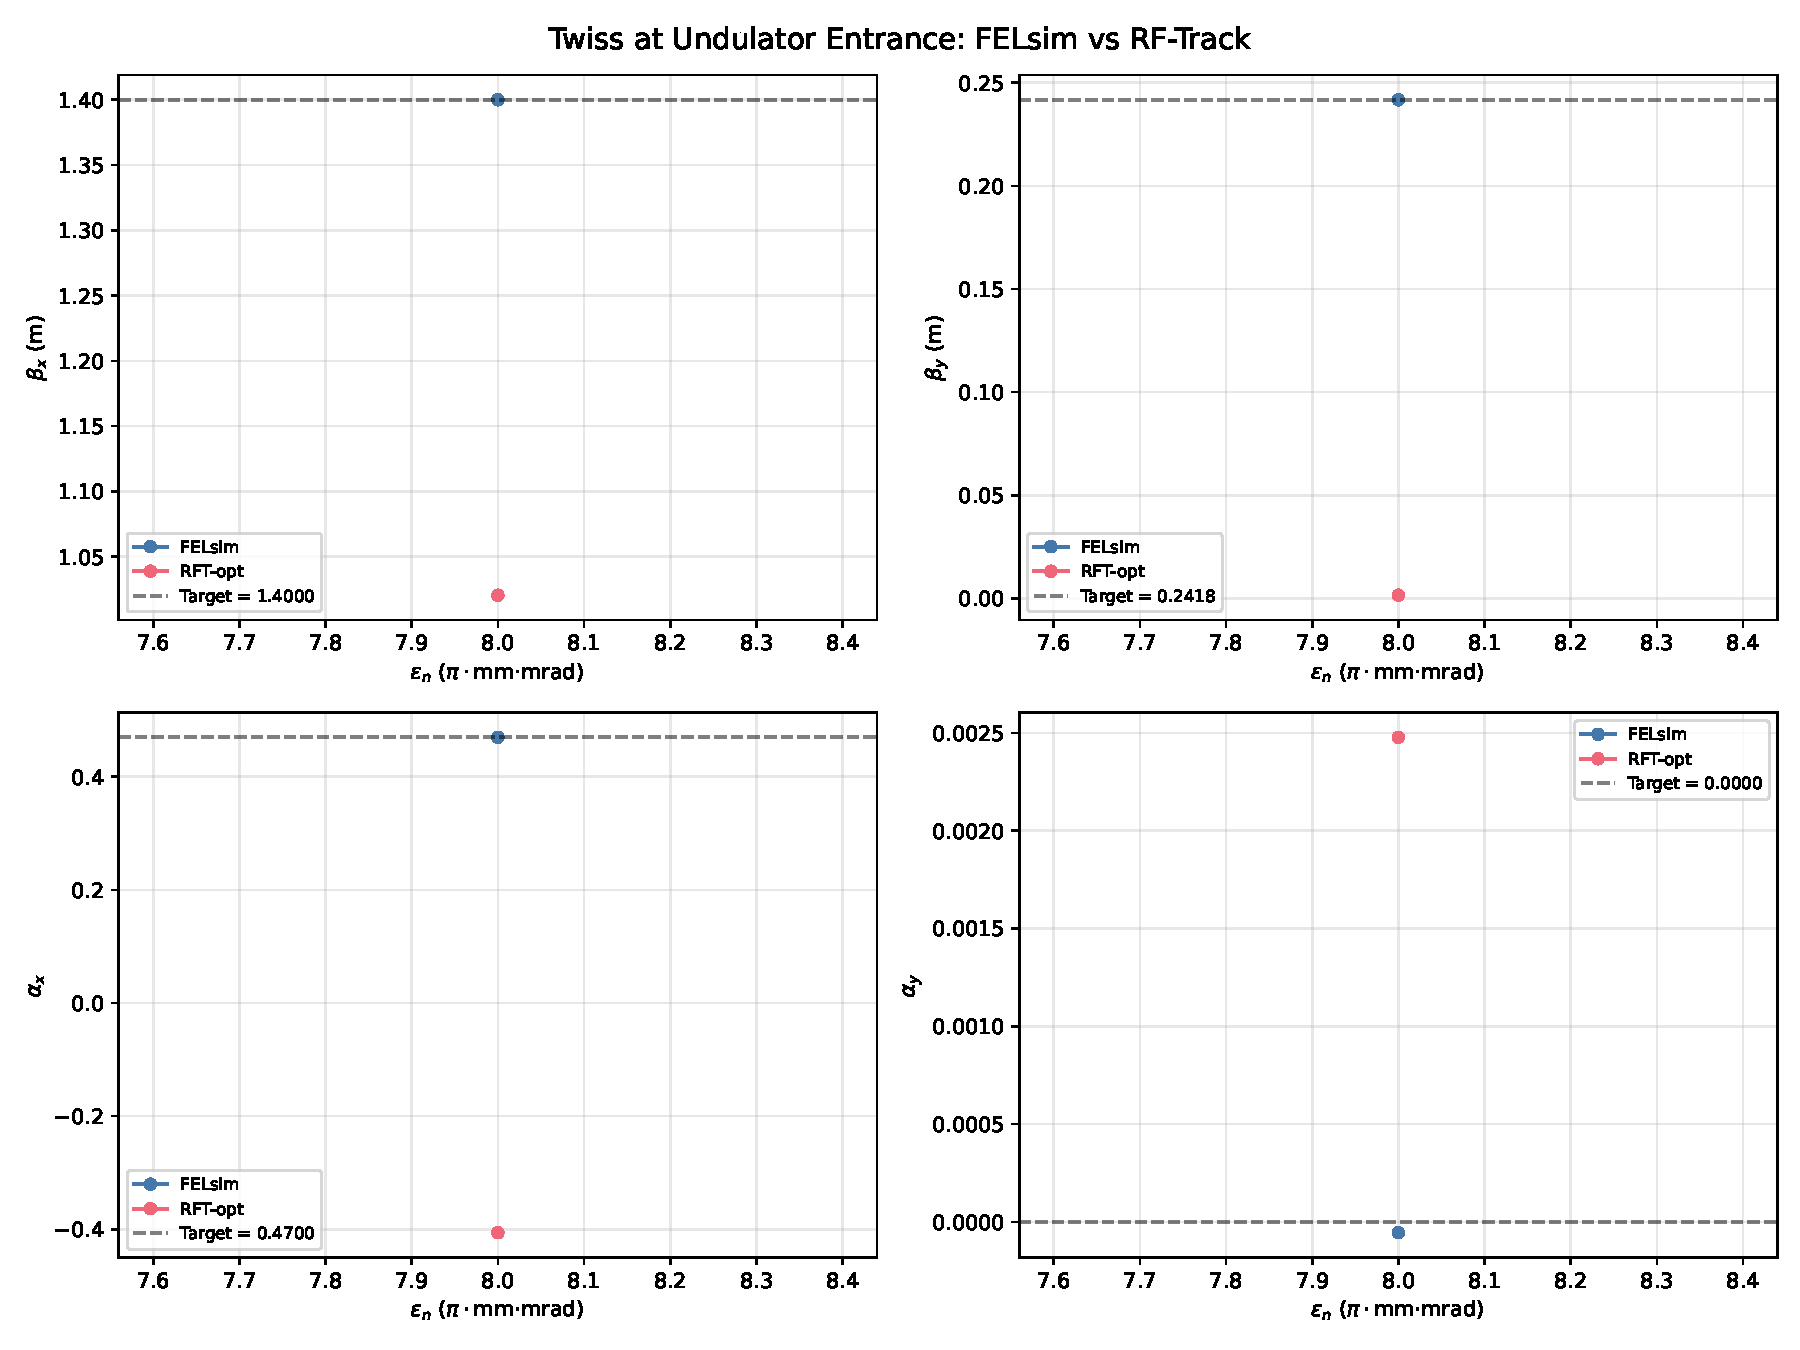
\includegraphics[width=0.85\textwidth]{results/rftrack_opt/twiss_comparison.pdf}
\caption{Twiss parameters at the undulator entrance.  Targets shown as
  dashed lines.  RFT-opt closely matches all targets; RFT-val diverges
  catastrophically.}
\label{fig:twiss}
\end{figure}


\section{Discussion}

\paragraph{Transfer of FELsim currents to RF-Track fails.}
The RFT-val result (MSE~$= 2552$, $\beta_x = 86$~m) demonstrates that
FELsim-optimised quad currents are not portable to RF-Track.
This is consistent with the W4 finding that currents cannot be exchanged
between codes with different dipole models: FELsim's triangle-rule fringe
correction and RF-Track's sector bend model produce different edge kicks at
each dipole, and these differences accumulate through 14~dipole sandwiches
(28~edge kicks) to shift the beam state far from the design orbit at
Stage~11.

\paragraph{RF-Track optimizer achieves $125\times$ better MSE.}
With 656 evaluations ($\approx$\SI{80}{s}), the RF-Track NM optimizer
converges to MSE~$= 6.4 \times 10^{-6}$, compared to FELsim's
$8.1 \times 10^{-4}$.  The two-order-of-magnitude improvement indicates that
RF-Track's particle-based Twiss computation provides a more precise match.
The FELsim MSE is limited by statistical noise in the target Twiss derivation
(computed from a finite particle distribution) and by linearization errors in
the transfer matrix model.

\paragraph{Different optimal currents.}
The RF-Track solution uses qualitatively different Stage~11 currents:
$I_{95} = 0.72$~A (vs.\ FELsim 2.89~A) and $I_{97} = 0.11$~A (vs.\ 1.92~A).
This is not surprising: the accumulated dipole model differences shift the
beam state arriving at Stage~11, requiring a different triplet correction.
Quads 93 and 87 remain similar (1.41 vs.\ 1.43~A, and 2.05 vs.\ 1.60~A),
suggesting the chromaticity quad and first triplet quad are less sensitive to
the upstream model differences.

\paragraph{Performance.}
Prefix caching makes RF-Track optimization practical: the
\SI{0.2}{s} prefix cost is amortised over 656 evaluations, each requiring
only two suffix trackings ($\approx$\SI{0.12}{s} per eval).  Total
optimisation time (\SI{80}{s}) is comparable to FELsim (\SI{82}{s}),
confirming that particle-tracking optimisation is feasible for routine use.


\section{Summary}

\begin{enumerate}
  \item FELsim-optimised Stage~11 currents produce incorrect optics in
    RF-Track (MSE~$= 2552$), confirming that currents are not portable
    between codes with different dipole edge models --- consistent with
    the COSY cross-validation~(W4).
  \item Re-optimising Stage~11 with RF-Track particle tracking achieves
    MSE~$= 6.4 \times 10^{-6}$, a $125\times$ improvement over FELsim's
    $8.1 \times 10^{-4}$.  Both codes can match the undulator Twiss targets,
    but each requires optimisation within its own physics model.
  \item Prefix caching (pre-tracking elements 0--87 once) makes
    particle-tracking optimisation practical: \SI{80}{s} total, comparable
    to FELsim.
  \item Two RF-Track adapter fixes were applied: \texttt{DIPOLE\_WEDGE}
    mapped to zero-length drift (instead of physical wedge length), and
    quadrupole \texttt{set\_strength()} confirmed correct despite ambiguous
    documentation.
\end{enumerate}

\paragraph{Next steps.}
\begin{itemize}
  \item Run the full emittance scan ($\varepsilon_n = 5, 8, 14$) with 5
    restarts to assess whether RF-Track resolves the $\varepsilon_n = 5$
    local-minimum problem identified in W2.
  \item Enable space charge in RF-Track to quantify collective effects
    on the undulator match.
  \item Compare RF-Track-optimised currents against the COSY FR\,1 solution
    (W4) for a three-code comparison at $\varepsilon_n = 8$.
\end{itemize}


\begin{thebibliography}{9}
\bibitem{weinberg2025}
  M.~Weinberg, A.~Fisher, and R.~Li,
  ``Design of the UH Mark V Free Electron Laser,''
  arXiv:2510.14061v1, Table~I.
\bibitem{rftrack}
  A.~Latina,
  \emph{RF-Track Reference Manual}, version~2.5.5,
  CERN, 2025.
\end{thebibliography}

\end{document}
